\section{Tokio}\label{sec:tokio}
Asynchronous programming in Rust requires an asynchronous run-time to poll the futures produced from \texttt{async}
functions.
One of the first run-times was Tokio~\citep{tokiocommunity_tokioasynchronousruntime_}, and has become the de-facto standard
asynchronous runtime for Rust.
Tokio existed prior to \asyncawait{} syntax as a runtime for futures directly.
At the beginning of the project, Rust was still stabilising its \asyncawait{} syntax~\citep{withoutboats_asyncawaitnotation_},
so there was no
complete and stable implementations of the asynchronous runtime.
The closest was Tokio's unstable implementation, which was stabilised soon after Rust stabilising
\asyncawait{}.
Now there exists multiple asynchronous run-times with the three main ones being Tokio, async-std and actix-rt.
Actix-rt provides an asynchronous runtime intended for use with the actor design pattern.
This API will not follow this pattern, so will not use actix-rt.
Async-std is a library which is modelled on Rust's own standard library with the intention of translating the standard
library to be \asyncawait{} compatible.
Where Tokio is intended to be a fully-featured asynchronous programming platform, async-std is a port of the existing
standard library.
Ultimately, Tokio is a more mature library with a much larger user base, so Tokio will be used over async-std.

\section{Connection Racing}\label{sec:connection-racing-impl}
As discussed in Section~\ref{sec:connection-racing}, the API must internally perform connection racing, utilising
Happy Eyeballs~\citep{pauly_happyeyeballsversion_}.
Using Rust's \texttt{Future} mechanism, the futures crate's \texttt{select\_ok()} method and both Tokio's task mechanism
and \texttt{delay\_for()} method, this can be implemented succinctly.

\begin{lstlisting}[float=h, label=fig:racer, caption={The connection racing implementation, with the delay on IPv4
        addresses.}]

async fn add_delay(addr: SocketAddr, props: Arc<TransportProperties>) -> Result<Connecting, Error> {
    match addr {
        SocketAddr::V4(_) => {
            time::delay_for(Duration::from_millis(5)).await
        }
        SocketAddr::V6(_) => time::delay_for(Duration::from_millis(0)).await,
    };
    Connecting::create(addr, props).await
}
pub async fn race<E, F>(
    endpoint: E,
    props: Arc<TransportProperties>,
    framer: F,
) -> Result<Box<dyn crate::Connection<F>>, Error>
where
    E: Endpoint,
    <E as Endpoint>::Error: 'static,
    F: Framer,
{
    ::futures::future::select_ok(
        endpoint
            .resolve()
            .await
            .map_err(box_error)
            .with_context(|| Resolve)?
            .map(|addr| task::spawn(add_delay(addr, props.clone())).boxed()),
    )
    .await
    .map(|x| x.0)
    .map_err(box_error)
    .with_context(|| Resolve)?
    .map(|x| x.framer(framer))
}
\end{lstlisting}

As shown in Listing~\ref{fig:racer}, the connection racing makes use of the \Endpoint{} trait to resolve the
endpoint before attempting to connect to each \texttt{SocketAddr}.
Each connection attempt future is executed using Tokio's task mechanism.
This is Tokio's asynchronous green threads implementation, which allows for each connection attempt to be conducted
simultaneously.
If Tokio's threaded runtime is enabled, the tasks are split across multiple threads, allowing for more concurrency over
Tokio's default runtime which is single threaded.
Without Tokio's task mechanism, each connection attempt will be done sequentially since they would all be executed as a
sequence of \texttt{Future}s.
An \texttt{await} can be viewed as a composition point of three \texttt{Futures}: the \texttt{Future} representing the
execution until the \texttt{await}, the \texttt{Future} be awaited and the \texttt{Future} following the \texttt{await}.
This produces code roughly equivalent to \lstinline{prior_future.and_then(awaiting_future).and_then(after_future)}.
Tokio's task mechanism ensures the \texttt{Future} it is given is executed concurrently to the \texttt{Future} it is
being composed with, allowing for a collection of concurrently executing \texttt{Future}s to be awaited with
\texttt{select\_ok()}.
The \texttt{select\_ok()} method takes an \texttt{Iterator} of \texttt{Future}s which resolve into \texttt{Result}, and
returns a \texttt{Future} which resolves into either the first of the given \texttt{Future}s to resolve into a
\texttt{Ok} and a list of the still executing \texttt{Future}s, or resolves into the last \texttt{Err} from the given
\texttt{Future}s.
The \texttt{map(|x| x.0)} drops the list of still executing \texttt{Future}s since they haven't won the race.

Tokio's \texttt{task::spawn()} function requires the \texttt{Future} it is given to have a \texttt{'static} definition.
This is generally best done through an \texttt{async} function which is defined outside of any scope, giving it a
\texttt{'static} lifetime.
For the \texttt{async} function's resulting \texttt{Future} to have a \texttt{'static} lifetime, it cannot have any
non-\texttt{'static} lifetime references in its arguments or return value.
If \texttt{add\_delay()}'s \texttt{props} argument was a reference to a \emph{TransportProperties}, Tokio's task
mechanism couldn't be used.
Through the use of an \texttt{Arc}\footnote{Atomic Reference Counting}, the \emph{TransportProperies} can be passed into
\texttt{add\_delay()} without cloning the whole object.
This is because \texttt{Arc}'s implementation of the \texttt{clone()} method is to create a new reference to the
underlying object and increment the reference count.
Avoiding cloning the \emph{TransportProperties} is beneficial because it could result in another heap allocation, which
would be detrimental for performance since this clone would have to done for each connection attempt.

The \emph{TransportProperties} doesn't have it's ownership given to the \texttt{race} function (passed by value),
because the \emph{TransportProperties} is stored in the \preconnection{} being used to create the \connection{}.
Since a \preconnection{} is a configuration object, it would be beneficial to be able to repeatedly create
\connection{}s from the same \preconnection{}.
Therefore, giving \texttt{race()} ownership of the \emph{TransportProperties} cannot be done as it would require
either cloning the \emph{TransportProperties} out of the \preconnection{} or also giving owership of the
\preconnection{}.
Instead, the \emph{TransportProperties} is stored within an \texttt{Arc} in the \preconnection{}, which is given to the
\texttt{race()} function.

During the race, a connection can either be connecting or connected, representing a racing connection and a winning
connection.
In the \texttt{add\_delay()} function, a connection attempt begins with \texttt{Connecting::create()} call.
Once a connection has one the race, it is converted into a \connection{} via the \texttt{x.framer()} call.
The \framer{} is not given to \texttt{Connecting}, because this would add an unnecessary \texttt{Clone} requirement to
all \framer{}s which are to be used with a \connection{}.
Rather, it is given to the \texttt{Connecting} which connected first, which converts itself into a \connection{}.

\section{Preconnection Endpoint Safety}\label{sec:preconnection-endpoint-safety}
As discussed in Section~\ref{subsec:preconnection}, a \preconnection{} can be given both local and remote endpoints.
A \connection{} and \listener{} require and can optionally make use of a different combination of local
and remote endpoints, as discussed in Section~\ref{subsec:connection} and Section~\ref{subsec:listener} respectively.
Two approaches to upholding these requirements exist: a runtime check which returns an error if a required endpoint is
not given, or a compile time check.
As discussed in Section~\ref{subsec:optional}, a compile time check is perferred as it prevents invalid code early in
the production cycle.

\begin{figure}[h]
    \centering
    \includegraphics[width=0.7\textwidth]{diagrams/preconn.png}
    \caption{A diagram to show Preconnection's endpoint statemachine.}
    \label{fig:preconState}
\end{figure}

To implement this check at compile time, the generic parameters \texttt{L} and \texttt{R} in the \preconnection{} struct
will be used to implement a state machine.
As showing in Figure~\ref{fig:preconState}, a \connection{} can only be created if the \preconnection{} has been given
a remote endpoint, and a \listener{} can only be created if the \preconnection{} has been given a local endpoint.
This is implemented by defining the marker (empty) trait \texttt{EndpointState}, which is implemented on the empty
struct \texttt{NoEndpoint} and any type which implements the \Endpoint{} trait.
Initially, both \texttt{L} and \texttt{R} are \texttt{NoEndpoint}, meaning the \preconnection{} is in the “No Endpoints”
state.
When a local endpoint or remote endpoint is given, \texttt{L} or \texttt{R} are set to the type of the given endpoint
respectively, and the state machine transitions to the “Local Endpoint Only” or “Remote Endpoint Only” state
respectively.
If the \preconnection{} is given the remaining unspecified endpoint, the state machine transitions to the
“Both Endpoints” state.
The \texttt{initiate()} method is only implemented if \texttt{R} implements the \Endpoint{} trait, which
\texttt{NoEndpoint} doesn't, therefore if the compiler allows a call to the \texttt{initiate()} method, a remote
endpoint must have be specified and the state machine is in either the “Remote Endpoint Only” or “Both Endpoints”
states.
Similarly, the \texttt{listen()} method is only implemented if \texttt{L} implements the endpoint trait, therefore
if a call to the \texttt{listen()} method is allowed by the compiler, a local endpoint must have been specified and the
state machine must be in either the “Local Endpoint Only” or “Both Endpoints” state.

%What did you do to implement this idea, and what technical achievements did you make?
%\section{Guidance}
%You can't talk about everything. Cover the high level first, then cover important, relevant or impressive details.
%
%
%
%\section{General points}
%
%These points apply to the whole dissertation, not just this chapter.
%
%
%
%\subsection{Figures}
%\emph{Always} refer to figures included, like Figure \ref{fig:relu}, in the body of the text. Include full, explanatory captions and make sure the figures look good on the page.
%You may include multiple figures in one float, as in Figure \ref{fig:synthetic}, using \texttt{subcaption}, which is enabled in the template.
%
%
%
%% Figures are important. Use them well.
%\begin{figure}
%    \centering
%    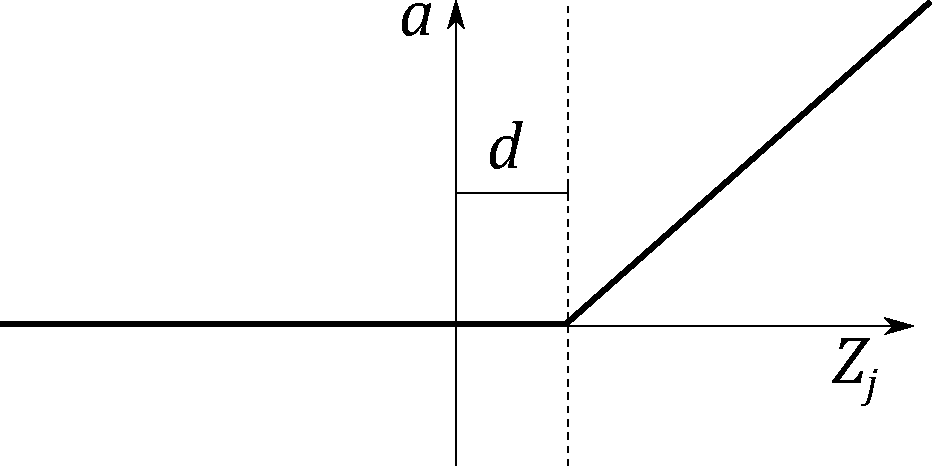
\includegraphics[width=0.5\linewidth]{images/relu.pdf}
%
%    \caption{In figure captions, explain what the reader is looking at: ``A schematic of the rectifying linear unit, where $a$ is the output amplitude,
%    $d$ is a configurable dead-zone, and $Z_j$ is the input signal'', as well as why the reader is looking at this:
%    ``It is notable that there is no activation \emph{at all} below 0, which explains our initial results.''
%    \textbf{Use vector image formats (.pdf) where possible}. Size figures appropriately, and do not make them over-large or too small to read.
%    }
%
%    % use the notation fig:name to cross reference a figure
%    \label{fig:relu}
%\end{figure}
%
%
%\begin{figure}
%    \centering
%    \begin{subfigure}[b]{0.45\textwidth}
%        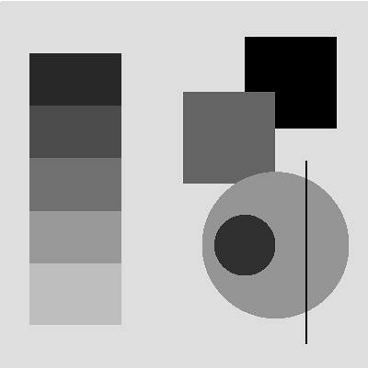
\includegraphics[width=\textwidth]{images/synthetic.png}
%        \caption{Synthetic image, black on white.}
%        \label{fig:syn1}
%    \end{subfigure}
%    ~ %add desired spacing between images, e. g. ~, \quad, \qquad, \hfill etc.
%      %(or a blank line to force the subfigure onto a new line)
%    \begin{subfigure}[b]{0.45\textwidth}
%        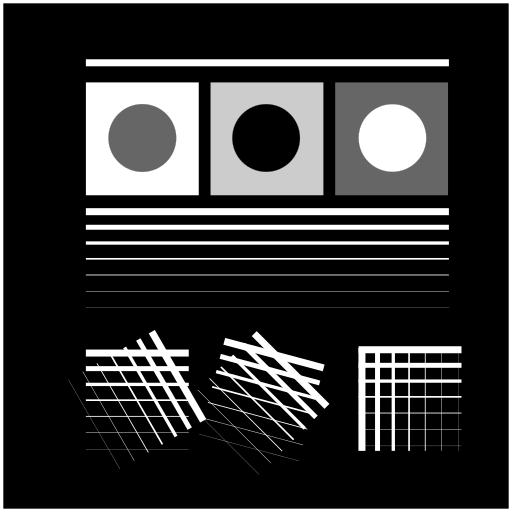
\includegraphics[width=\textwidth]{images/synthetic_2.png}
%        \caption{Synthetic image, white on black.}
%        \label{fig:syn2}
%    \end{subfigure}
%    ~ %add desired spacing between images, e. g. ~, \quad, \qquad, \hfill etc.
%    %(or a blank line to force the subfigure onto a new line)
%    \caption{Synthetic test images for edge detection algorithms. \subref{fig:syn1} shows various gray levels that require an adaptive algorithm. \subref{fig:syn2}
%    shows more challenging edge detection tests that have crossing lines. Fusing these into full segments typically requires algorithms like the Hough transform.
%    This is an example of using subfigures, with \texttt{subref}s in the caption.
%    }\label{fig:synthetic}
%\end{figure}
%
%\clearpage
%
%\subsection{Equations}
%
%Equations should be typeset correctly and precisely. Make sure you get parenthesis sizing correct, and punctuate equations correctly
%(the comma is important and goes \textit{inside} the equation block). Explain any symbols used clearly if not defined earlier.
%
%For example, we might define:
%\begin{equation}
%    \hat{f}(\xi) = \frac{1}{2}\left[ \int_{-\infty}^{\infty} f(x) e^{2\pi i x \xi} \right],
%\end{equation}
%where $\hat{f}(\xi)$ is the Fourier transform of the time domain signal $f(x)$.
%
%\subsection{Algorithms}
%Algorithms can be set using \texttt{algorithm2e}, as in Algorithm \ref{alg:metropolis}.
%
%% NOTE: line ends are denoted by \; in algorithm2e
%\begin{algorithm}
%    \DontPrintSemicolon
%    \KwData{$f_X(x)$, a probability density function returing the density at $x$.\; $\sigma$ a standard deviation specifying the spread of the proposal distribution.\;
%    $x_0$, an initial starting condition.}
%    \KwResult{$s=[x_1, x_2, \dots, x_n]$, $n$ samples approximately drawn from a distribution with PDF $f_X(x)$.}
%    \Begin{
%        $s \longleftarrow []$\;
%        $p \longleftarrow f_X(x)$\;
%        $i \longleftarrow 0$\;
%        \While{$i < n$}
%        {
%            $x^\prime \longleftarrow \mathcal{N}(x, \sigma^2)$\;
%            $p^\prime \longleftarrow f_X(x^\prime)$\;
%            $a \longleftarrow \frac{p^\prime}{p}$\;
%            $r \longleftarrow U(0,1)$\;
%            \If{$r<a$}
%            {
%                $x \longleftarrow x^\prime$\;
%                $p \longleftarrow f_X(x)$\;
%                $i \longleftarrow i+1$\;
%                append $x$ to $s$\;
%            }
%        }
%    }
%
%\caption{The Metropolis-Hastings MCMC algorithm for drawing samples from arbitrary probability distributions,
%specialised for normal proposal distributions $q(x^\prime|x) = \mathcal{N}(x, \sigma^2)$. The symmetry of the normal distribution means the acceptance rule takes the simplified form.}\label{alg:metropolis}
%\end{algorithm}
